%==============================================================================
% Sjabloon poster bachproef
%==============================================================================
% Gebaseerd op document class `a0poster' door Gerlinde Kettl en Matthias Weiser
% Aangepast voor gebruik aan HOGENT door Jens Buysse en Bert Van Vreckem

\documentclass[a0,portrait]{hogent-poster}

% Info over de opleiding
\course{Bachelorproef}
\studyprogramme{toegepaste informatica}
\academicyear{2023-2024}
\institution{Hogeschool Gent, Valentin Vaerwyckweg 1, 9000 Gent}

% Info over de bachelorproef
\title{Hoe kan Machine Learning/Artificial Intelligence gebruikt worden om de kwaliteit van artikel data te verhogen?}
%\subtitle{Ondertitel (eventueel)}
\author{Maëlys Callens}
\email{maelys.callens@student.hogent.be}
\supervisor{Sebastiaan Labijn}
\cosupervisor{Nicholas Vermeersch (Alluvion)}

% Indien ingevuld, wordt deze informatie toegevoegd aan het einde van de
% abstract. Zet in commentaar als je dit niet wilt.
\specialisation{Machineleertechnieken en artificiële intelligentie}
\keywords{ERP, master data, artikel data, Python}
\projectrepo{https://github.com/MaelysCallens/2324_BAP.git}

\begin{document}

\maketitle

\begin{abstract}
In een tijd waarin bedrijven steeds meer data genereren en gebruiken, is het verbeteren van de kwaliteit van gegevens essentieel geworden voor een succesvolle bedrijfsvoering. Dit geldt met name voor master data, die fungeren als de kern van operationele processen, besluitvorming en klantinteracties. Ondanks het belang ervan blijft het beheer van master data een uitdagend vraagstuk vanwege problemen zoals inconsistentie en duplicatie. Machine Learning (ML) en Artificial Intelligence (AI) worden steeds belangrijker omdat ze krachtige instrumenten bieden om de kwaliteit en bruikbaarheid van gegevens te verbeteren.
  \\
Het doel van dit onderzoek is om methoden en technieken te identificeren die organisaties kunnen toepassen om de kwaliteit van artikel data te verbeteren door ML en AI te benutten. Een proof-of-concept wordt ontwikkeld om een model te creëren dat de kwaliteit van artikel data kan verbeteren door een duplicaatdetectiesysteem op te stellen, waardoor het gebruikersproces wordt gestroomlijnd en de kans op fouten wordt verminderd. 
  \\
Het onderzoek draagt bij aan de optimalisatie van gegevensbeheer binnen moderne bedrijfsomgevingen, waardoor organisaties beter gebruik kunnen maken van hun waardevolle bedrijfsgegevens.
\end{abstract}

\begin{multicols}{2} % This is how many columns your poster will be broken into, a portrait poster is generally split into 2 columns

\section{Introductie}

In een tijdperk waarin data als het nieuwe goud beschouwd wordt, staat het optimaliseren van de gegevenskwaliteit centraal in het streven naar een succesvolle bedrijfsvoering. Door de exponentiële groei van informatie binnenin organisaties, voornamelijk door Enterprise Resource Planning (ERP) systemen, wordt de essentiële rol van het beheren en het verrijken van master data benadrukt. Deze gegevens vormen de ruggengraat van de operationele processen, de besluitvorming en de klantinteracties. Hierdoor wordt hun accuraatheid en consistentie van vitaal belang voor organisatorische efficiëntie en concurrentievoordeel.
\\
Echter, in de bedrijfsomgevingen blijft het beheer van master data een complex en uitdagend vraagstuk. Het gebrek aan uniformiteit, de aanwezigheid van duplicaten en de inconsistente gegevensformaten vormen obstakels voor een effectief gegevensbeheer. Dit leidt dan tot fouten, inefficiënties en gemiste kansen voor bedrijven om waarde uit hun gegevens te halen. 
\\
Hierbij is de rol van Machine Learning (ML) en Artificial Intelligence (AI) steeds belangrijker geworden. Deze technologieën bieden krachtige instrumenten om de kwaliteit en de bruikbaarheid van gegevens te verbeteren. Door het vermogen om patronen te identificeren, trends te voorspellen en complexe taken uit te voeren, bieden ML en AI een veelbelovend perspectief voor het verhogen van de waarde die uit de data gehaald kan worden.

\section{Onderzoek}

In deze studie wordt eerst een onderzoek gedaan naar de vereisten waaraan een duplicaat detectie systeem moet voldoet. Vervolgens worden diverse tools geanalyseerd en besproken op basis van deze requirements. De tools die in deze bachelorproef worden besproken zijn SAP, SAP Master Data Governance, Syniti Match, IBM Info Sphere Master Data Management, Pimcore Product Information Management en Pimcore Customer Management Framework. Aan de hand van deze requirementsanalyse is het proof-of-concept opgesteld. Er is een model ontwikkeld met behulp van ML en AI. Als eerste wordt er een dataset van 5 000 records van artikel data verwerkt en klaargemaakt om het model te trainen. Daarna deelt het model de records op in drie verschillende groepen die gelijkenissen met elkaar vertonen. Als laatste stap is het effectieve duplicaatdetectiesysteem opgezet en worden de duplicaten geanalyseerd. 

%\section{Sectie met figuur}


\begin{center}
  \captionsetup{type=figure}
  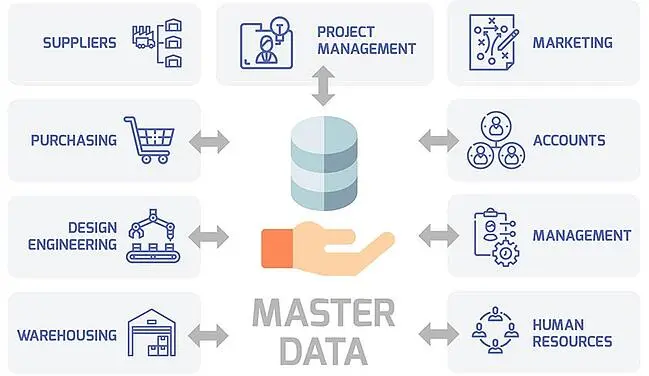
\includegraphics[width=1.0\linewidth]{../images/Master-Data.png}
  \captionof{figure}{Master Data}
\end{center}


\section{Conclusies}

Tijdens deze studie zijn er verschillende vereisten opgesteld door middel van een requirementsanalyse. Door deze requirements op te stellen, is er onderzoek verricht naar diverse tools die instaan voor duplicaat detectie. Deze tools zijn beoordeeld op basis van de vooropgestelde requirements. In het proof-of-concept is een duplicaat detectie gebouwd. Het model biedt een basis waarmee duplicaten gedetecteerd kunnen worden in een bestaande dataset. Het kan ook op nieuwe data toegepast worden en is daarnaast ontworpen om te blijven leren van andere data, zodat het model geoptimaliseerd kan worden. Het verder onderzoeken en testen van nieuwe algoritmen op vlak van clustering en duplicaat detectie kan voor nog betere resultaten zorgen. Uit deze studie blijkt dat Artificiële Intelligentie en Machine Learning significant kunnen bijdragen aan de verbetering van de kwaliteit van artikel data. 

\section{Toekomstig onderzoek}

De bevindingen van dit onderzoek kunnen als een stimulans dienen voor verdere verkenning en verbetering van de huidige algoritmen die worden gebruikt voor duplicaat detectie bij master data. De voordelen van kunstmatige intelligentie in dit domein zijn duidelijk aangetoond, wat de optimalisatie van deze technologieën en hun naadloze integratie met master data management systemen, zoals SAP Master Data Governance, essentieel maakt. Bedrijven die streven naar hogere en betere datakwaliteit kunnen door deze resultaten worden aangemoedigd om machine learning-modellen te implementeren. 

\end{multicols}
\end{document}